\section{Ćwiczenia 4: 16-III-2017}
\subsection{Zadania Domowe A}
Uwaga: We wszystkich zadaniach A oznacza macierz przyległości rozważanego w zadaniu grafu. Przez przekątna macierzy rozumiemy jej główna przekątna.			
\paragraph{A1}
\begin{figure}[H]
%\begin{wrapfigure}{r}{0.3\textwidth}
\centering
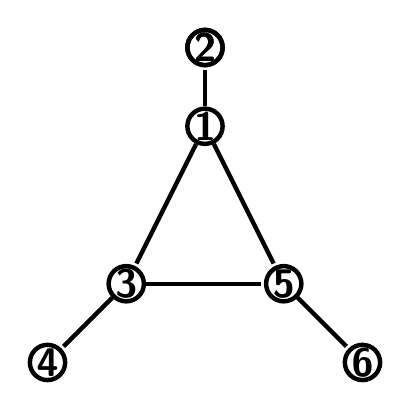
\begin{tikzpicture}[shorten >=1pt, auto, node distance=3cm, ultra thick,main node/.style={circle,draw,minimum size=.4cm,inner sep=0pt]}]%fill=black,
\begin{scope}[every node/.style={font=\sffamily\Large\bfseries}]
\node[main node] (v4) at (0,0) {4};
\node[main node] (v3) at (1,1) {3};
\node[main node] (v1) at (2,3) {1};
\node[main node] (v2) at (2,4) {2};
\node[main node] (v5) at (3,1) {5};
\node[main node] (v6) at (4,0) {6};
\node[main node] (v7) at (2,4) {2};
%\node[main node] (v) at (,) {};
\end{scope}
\begin{scope}
\draw  (v1) edge node{} (v2);
\draw  (v1) edge node{} (v3);
\draw  (v1) edge node{} (v5);
\draw  (v3) edge node{} (v4);
\draw  (v3) edge node{} (v5);
\draw  (v5) edge node{} (v6);
%\draw  (v) edge node{} (v);
\end{scope}
\end{tikzpicture}
\caption*{Graf $G$.}
%\end{wrapfigure}
\end{figure}

\begin{enumerate}[label=\arabic*)]
\item Rozważmy narysowany obok graf $G$.
\begin{enumerate}[label=\alph*)]
\item Ile jest spacerów długości $3$ wierzchołka $1$ do $1$?

\textbf{Odpowiedź: }$A^3\rightarrow a_{1,1}=2$
\item Ile jest wszystkich spacerów zamkniętych	długości $3$ w grafie $G$?\\
Spacer zamknięty taki, który zaczyna się i kończy w tym samym wierzchołku.		

\textbf{Odpowiedź: }$A^3\rightarrow \sum_{i=1}^n a_{i,i}=6$
\item Nie podnosząc do potęgi macierzy  $A$,  opisz  główną przekątna macierzy $A^3$.

\textbf{Odpowiedź: }Główna przekątna macierzy $A^3$ zawiera ilość ścieżek o długości $3$ od i do ,,wierzchołka startowego'' czyli dla wierzchołków: $1,3,5$ jest wartość $2$, $0$ w pozostałych przepadkach.
\end{enumerate}

\item Załóżmy, że $G$ jest ścieżką o $6$ wierzchołkach, ponumerowanych kolejno $1,2,3,4,5,6$.
\begin{figure}[H]
\centering
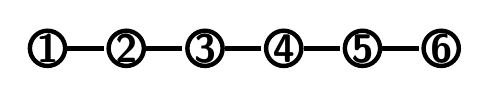
\begin{tikzpicture}[shorten >=1pt, auto, node distance=3cm, ultra thick,main node/.style={circle,draw,minimum size=.4cm,inner sep=0pt]}]%fill=black,
\begin{scope}[every node/.style={font=\sffamily\Large\bfseries}]
\node[main node] (v1) at (0,0) {1};
\node[main node] (v2) at (1,0) {2};
\node[main node] (v3) at (2,0) {3};
\node[main node] (v4) at (3,0) {4};
\node[main node] (v5) at (4,0) {5};
\node[main node] (v6) at (5,0) {6};
%\node[main node] (v) at (,) {};
\end{scope}
\begin{scope}
\draw  (v1) edge node{} (v2);
\draw  (v2) edge node{} (v3);
\draw  (v3) edge node{} (v4);
\draw  (v4) edge node{} (v5);
\draw  (v5) edge node{} (v6);
%\draw  (v) edge node{} (v);
\end{scope}
\end{tikzpicture}
\caption*{Graf $G$.}
\end{figure}
\begin{enumerate}[label=\alph*)]
\item Ile jest spacerów długości $3$ z wierzchołka $1$ do $2$? 

\textbf{Odpowiedź: }$2$: $1\rightarrow 2\rightarrow 1\rightarrow 2$ i $1\rightarrow 2\rightarrow 3\rightarrow 2$
\item Ile jest spacerów długości $7$ z wierzchołka $1$ do $6$? 
=
\textbf{Odpowiedź: } $5$
\item Ile jest spacerów długości $100$ z wierzchołka $1$ do $6$?

\textbf{Odpowiedź: } $0$
\item Ile jest spacerów długości $101$ z wierzchołka $1$ do $1$?

\textbf{Odpowiedź: }$0$
\item Jaki jest wyraz w pierwszym wierszu i szóstej kolumnie macierzy $A^7$? 

\textbf{Odpowiedź: } $$A^7=\begin{bmatrix}
0&14&0&14&0&5\\
14&0&28&0&19&0\\
0&28&0&33&0&14\\
14&0&33&0&28&0\\
0&19&0&28&0&14\\
5&0&14&0&14&0
\end{bmatrix}$$
\item Jak wygląda przekątna macierzy $A^{101}$? 

\textbf{Odpowiedź: }Zera
\end{enumerate}
\item W drzewie $T$ na $17$ wierzchołkach, wierzchołek numer $3$ ma stopień $4$, wierzchołek numer $7$ ma stopień $5$. Ponadto wierzchołki $3$ i $7$ są przylegle. Znajdź wyraz w trzecim wierszu i siódmej kolumnie macierzy $A^3$. 

\textbf{Odpowiedź: }
\begin{figure}[H]
\centering
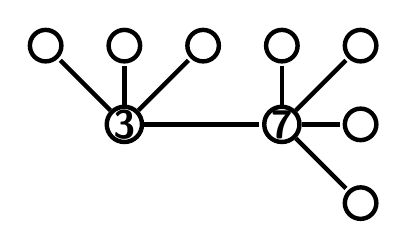
\begin{tikzpicture}[shorten >=1pt, auto, node distance=3cm, ultra thick,main node/.style={circle,draw,minimum size=.4cm,inner sep=0pt]}]%fill=black,
\begin{scope}[every node/.style={font=\sffamily\Large\bfseries}]
\node[main node] (v31) at (0,1) {};
\node[main node] (v32) at (1,1) {};
\node[main node] (v33) at (2,1) {};
\node[main node] (v3) at (1,0) {3};
\node[main node] (v7) at (3,0) {7};
\node[main node] (v71) at (3,1) {};
\node[main node] (v72) at (4,1) {};
\node[main node] (v73) at (4,0) {};
\node[main node] (v74) at (4,-1) {};

%\node[main node] (v) at (,) {};
\end{scope}
\begin{scope}
\draw  (v3) edge node{} (v7);
\draw  (v3) edge node{} (v31);
\draw  (v3) edge node{} (v32);
\draw  (v3) edge node{} (v33);
\draw  (v7) edge node{} (v71);
\draw  (v7) edge node{} (v72);
\draw  (v7) edge node{} (v73);
\draw  (v7) edge node{} (v74);
%\draw  (v) edge node{} (v);
\end{scope}
\end{tikzpicture}
\caption*{Graf $G$.}
\end{figure}
$V(T)=17,\ \deg (3)=4,\ \deg (7)=5,\ \{3,7\}\in E(T)$
$$A^3\rightarrow a_{3,7}=8\Rightarrow \deg (3) + \deg (7) - 1=4+5-1=8$$

\item Czy z faktu, że wszystkie wyrazy na głównej przekątnej macierzy $A^4$ są zerami wynika, że w grafie nie ma cykli na $4$ wierzchołkach?

\textbf{Odpowiedź: }Wynika, że nie ma spacerów o długości $4$ które zaczynałyby się i kończyły w tym samym wierzchołku.
\end{enumerate}
	
\paragraph{A2}
\begin{figure}[H]
%\begin{wrapfigure}{r}{0.3\textwidth}
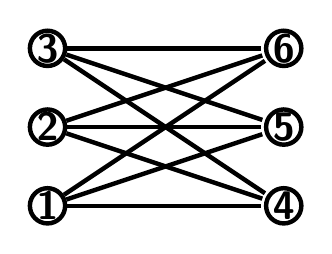
\begin{tikzpicture}[shorten >=1pt, auto, node distance=3cm, ultra thick,main node/.style={circle,draw,minimum size=.4cm,inner sep=0pt]}]%fill=black,
\begin{scope}[every node/.style={font=\sffamily\Large\bfseries}]
\node[main node] (v1) at (0,0) {1};
\node[main node] (v2) at (0,1) {2};
\node[main node] (v3) at (0,2) {3};
\node[main node] (v4) at (3,0) {4};
\node[main node] (v5) at (3,1) {5};
\node[main node] (v6) at (3,2) {6};
%\node[main node] (v) at (,) {};
\end{scope}
\begin{scope}
\draw  (v1) edge node{} (v4);
\draw  (v1) edge node{} (v5);
\draw  (v1) edge node{} (v6);
\draw  (v2) edge node{} (v4);
\draw  (v2) edge node{} (v5);
\draw  (v2) edge node{} (v6);
\draw  (v3) edge node{} (v4);
\draw  (v3) edge node{} (v5);
\draw  (v3) edge node{} (v6);
%\draw  (v) edge node{} (v);
\end{scope}
\end{tikzpicture}
\caption*{Graf $K_{3,3}$.}
%\end{wrapfigure}
\end{figure}

\begin{enumerate}[label=\alph*)]
\item Wyznacz $A^3$ dla grafu $K_{3,3}$.

$$A=\begin{bmatrix}
0&0&0&1&1&1\\
0&0&0&1&1&1\\
0&0&0&1&1&1\\
1&1&1&0&0&0\\
1&1&1&0&0&0\\
1&1&1&0&0&0
\end{bmatrix}$$
$$A^3=\begin{bmatrix}
0&0&0&9&9&9\\
0&0&0&9&9&9\\
0&0&0&9&9&9\\
9&9&9&0&0&0\\
9&9&9&0&0&0\\
9&9&9&0&0&0
\end{bmatrix}$$
\item Wyznacz $A^3$ dla grafu $K_{N,N}$, nie wykonując żadnych mnożeń macierzy.

$$A^3(K_{N,N})=\left\{\begin{matrix}
0 & \text{ dla }2\text{ i }4 \text{ ćwiartki macierzy}\\
N^2 & \text{ dla }1\text{ i }3 \text{ ćwiartki macierzy}
\end{matrix}\right.$$
\item Wyznacz $A^2$ dla grafu $K_{N,N}$.

$$A^2(K_{N,N})=\left\{\begin{matrix}
N & \text{ dla }2\text{ i }4 \text{ ćwiartki macierzy}\\
0 & \text{ dla }1\text{ i }3 \text{ ćwiartki macierzy}
\end{matrix}\right.$$
\end{enumerate}

\paragraph{A3} Załóżmy, że $G$ jest grafem $5$– regularnym o $100$ wierzchołkach.
\begin{enumerate}[label=\alph*)]
\item Ile jest w $G$ cykli długości $4$, zawierających wierzchołek numer $1$, jeżeli na pierwszym miejscu przekątnej macierzy $A^4$ stoi liczba $55$?

\textbf{Odpowiedź: }Możliwe ścieżki długości 4:\\
\begin{minipage}{.25\textwidth}
\begin{figure}[H]\centering
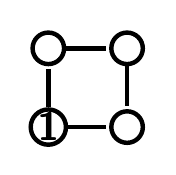
\begin{tikzpicture}[shorten >=1pt, auto, node distance=3cm, ultra thick,main node/.style={circle,draw,minimum size=.4cm,inner sep=0pt]}]%fill=black,
\begin{scope}[every node/.style={font=\sffamily\Large\bfseries}]
\node[main node] (v1) at (0,0) {1};
\node[main node] (v2) at (0,1) {};
\node[main node] (v3) at (1,1) {};
\node[main node] (v4) at (1,0) {};
%\node[main node] (v) at (,) {};
\end{scope}
\begin{scope}
\draw  (v1) edge node{} (v2);
\draw  (v1) edge node{} (v4);
\draw  (v2) edge node{} (v3);
\draw  (v3) edge node{} (v4);
%\draw  (v) edge node{} (v);
\end{scope}
\end{tikzpicture}
\caption*{I\newline $1\rightarrow 2\rightarrow 3\rightarrow 4\rightarrow 1$\newline $1\rightarrow 4\rightarrow 3\rightarrow 2\rightarrow 1$\newline $2*5=10$ możliwości}
\end{figure}
\end{minipage}
\begin{minipage}{.25\textwidth}
\begin{figure}[H]\centering
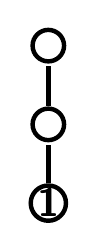
\begin{tikzpicture}[shorten >=1pt, auto, node distance=3cm, ultra thick,main node/.style={circle,draw,minimum size=.4cm,inner sep=0pt]}]%fill=black,
\begin{scope}[every node/.style={font=\sffamily\Large\bfseries}]
\node[main node] (v1) at (0,0) {1};
\node[main node] (v2) at (0,1) {};
\node[main node] (v3) at (0,2) {};
%\node[main node] (v) at (,) {};
\end{scope}
\begin{scope}
\draw  (v1) edge node{} (v2);
\draw  (v2) edge node{} (v3);
%\draw  (v) edge node{} (v);
\end{scope}
\end{tikzpicture}
\caption*{II\newline $1\rightarrow 2\rightarrow 3\rightarrow 2\rightarrow 1$\newline $5*4=20$ możliwości}
\end{figure}
\end{minipage}
\begin{minipage}{.25\textwidth}
\begin{figure}[H]\centering
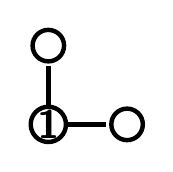
\begin{tikzpicture}[shorten >=1pt, auto, node distance=3cm, ultra thick,main node/.style={circle,draw,minimum size=.4cm,inner sep=0pt]}]%fill=black,
\begin{scope}[every node/.style={font=\sffamily\Large\bfseries}]
\node[main node] (v1) at (0,0) {1};
\node[main node] (v2) at (0,1) {};
\node[main node] (v3) at (1,0) {};
%\node[main node] (v) at (,) {};
\end{scope}
\begin{scope}
\draw  (v1) edge node{} (v2);
\draw  (v1) edge node{} (v3);
%\draw  (v) edge node{} (v);
\end{scope}
\end{tikzpicture}
\caption*{III\newline $1\rightarrow 2\rightarrow 1\rightarrow 3\rightarrow 1$\newline $5*4=20$ możliwości}
\end{figure}
\end{minipage}
\begin{minipage}{.25\textwidth}
\begin{figure}[H]
\centering
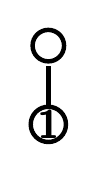
\begin{tikzpicture}[shorten >=1pt, auto, node distance=3cm, ultra thick,main node/.style={circle,draw,minimum size=.4cm,inner sep=0pt]}]%fill=black,
\begin{scope}[every node/.style={font=\sffamily\Large\bfseries}]
\node[main node] (v1) at (0,0) {1};
\node[main node] (v2) at (0,1) {};
%\node[main node] (v) at (,) {};
\end{scope}
\begin{scope}
\draw  (v1) edge node{} (v2);
%\draw  (v) edge node{} (v);
\end{scope}
\end{tikzpicture}
\caption*{IV\newline $1\rightarrow 2\rightarrow 1\rightarrow 2\rightarrow 1$\newline $5$ możliwości}
\end{figure}
\end{minipage}
$$5+20+20+10=55$$
Interesują nas tylko ścieżki określone sposobem I ale że w cyklu nie ważna jest kolejność (tylko sam cykl) także odpowiedź to $\frac{10}{2}=5$. 

\item Ile jest w $G$ cykli długości $4$, jeżeli wszystkie wyrazy na przekątnej	macierzy $A^4$ wynoszą $45$?

\textbf{Odpowiedź: }Brak takich cykli, zgonie z ,,możliwymi'' kombinacjami ścieżek (przy grafie 5-regularnym) i sumując opcję: IV + III + II uzyskujemy 45.
\todo[inline,color=red]{SPRAWDZIĆ ZADANIE.}
\item Ile jest w $G$ cykli długości $4$, jeżeli $\mathsf{Tr}(A^4) = 4900$?

\textbf{Odpowiedź: }Możemy zapisać jako:
\begin{align*}
& 5*100 \tag*{Zgodnie z możliwą ścieżką nr IV}\\ 
&+ 2*100 \tag*{ścieżka nr III}\\ 
&+ 20*100 \tag*{ścieżka nr II}\\ 
&+ 2*4*x \tag*{ścieżka nr I i poszukiwana wartość $x$ - liczba cykli} \\ 
&= 4900\\
& 500+2000+2000+8x=4900 \\
& 8x = 400\\
& x = 50
\end{align*}
W grafie $G$ cykli o długości $4$, jeżeli $\mathsf{Tr}(A^4) = 4900$, jest $50$.
\end{enumerate}

\paragraph{A4}
Niech
$$B = \begin{bmatrix}
-1 & -4\\
 2 & 5
\end{bmatrix},\ C=\begin{bmatrix}
-1 & -4& 0\\
2&5&0\\
0&0&3
\end{bmatrix}$$
\begin{enumerate}[label=\alph*)]
\item Czy $\begin{bmatrix}
1\\-1
\end{bmatrix}$ jest wektorem własnym macierzy $B$?
\item Czy $\begin{bmatrix}
2\\1
\end{bmatrix}$ jest wektorem własnym macierzy $B$?
\item Czy $-3$ jest wartością własną macierzy $B$? 

\textbf{Odpowiedź: } Dwie metody  
\begin{enumerate}[label=\Roman*:]
\item Wyliczyć:
\begin{align*}
&B_\lambda = \begin{bmatrix}
-1 & -4\\ 2 & 5
\end{bmatrix} - \lambda \begin{bmatrix}
1&0\\0&1
\end{bmatrix}=\begin{bmatrix}
-1-\lambda&-4\\
2&5-\lambda
\end{bmatrix}\\
&\begin{vmatrix}
-1-\lambda&-4\\
2&5-\lambda
\end{vmatrix}=(-1\lambda )(5-\lambda )-(2*-4)=\lambda ^2-4\lambda +3\\
&\Delta = (-4)^2-4*1*3=4\\
&\lambda _1 = 1\ \lambda _2 =3\\
&B_{\lambda _1}= \begin{bmatrix}
-2 & -4\\ 2 & 4
\end{bmatrix} \Rightarrow \begin{bmatrix}
-2 & -4\\ 2 & 4
\end{bmatrix} \begin{bmatrix}
x\\y
\end{bmatrix}=\begin{bmatrix}
0\\0
\end{bmatrix}\\
&\left\{\begin{matrix}
-2x &-4u &= 0\\
2x &+ 4y &= 0
\end{matrix}\right. \Rightarrow -2x = 4y\Rightarrow -x=2y \Rightarrow \begin{bmatrix}
-1 \\2
\end{bmatrix}\\
%-------
&B_{\lambda _2}= \begin{bmatrix}
-4 & -4\\ 2 & 2
\end{bmatrix} \Rightarrow \begin{bmatrix}
-4 & -4\\ 2 & 2
\end{bmatrix} \begin{bmatrix}
x\\y
\end{bmatrix}=\begin{bmatrix}
0\\0
\end{bmatrix}\\
&\left\{\begin{matrix}
-4x &-4y &= 0\\
2x &+ 2y &= 0
\end{matrix}\right. \Rightarrow x=-y \Rightarrow \begin{bmatrix}
1\\-1
\end{bmatrix}
\end{align*}
\begin{enumerate}[label=\alph*)]
\item TAK
\item NIE
\item NIE
\end{enumerate}
\item (mądrzej) wymnożyć
\begin{align*}
&\begin{bmatrix}
-1 & -4\\
2 & 5
\end{bmatrix} * \begin{bmatrix}
1\\-1
\end{bmatrix}=\begin{bmatrix}
-1*1+-4*-1\\
2*1+5*-1
\end{bmatrix}= \begin{bmatrix}
3\\
-3
\end{bmatrix}=3\begin{bmatrix}
1\\-1
\end{bmatrix} \\
& \begin{bmatrix}
-1 & -4\\
2 & 5
\end{bmatrix} * \begin{bmatrix}
2\\1
\end{bmatrix} = \begin{bmatrix}
-1*2+-4*1 \\
2*2+5*1
\end{bmatrix} = \begin{bmatrix}
-6\\
9
\end{bmatrix}=3*\begin{bmatrix}
-2\\3
\end{bmatrix}
\end{align*}

\end{enumerate}
\item Czy $\begin{bmatrix}
1\\-1\\1
\end{bmatrix}$jest wektorem własnym macierzy $C$?
\item Czy $0$ jest wartością własną macierzy $C$? 

\textbf{Odpowiedź:}
\begin{enumerate}[label=\alph*)]
\item Nie, wektorami własnymi są:
$$\begin{bmatrix}
-1\\1\\0
\end{bmatrix}\ \begin{bmatrix}
-2\\1\\0
\end{bmatrix}\ \begin{bmatrix}
0\\0\\1
\end{bmatrix}$$
\item Nie! Wartościami własnymi są:
$$\lambda _1 = 1,\, \lambda _{2,3}=3\footnotemark$$
\footnotetext{$\Delta$ była równa 0}
\end{enumerate}
\end{enumerate}

\paragraph{A5} Bohaterem tego zadania jest graf $K_3$.
\begin{enumerate}[label=\alph*)]
\item Wyznacz $A^2$, $A^3$ i $A^4$. Na tej podstawie oblicz ślady macierzy $A^2$, $A^3$ i $A^4$.

\textbf{Odpowiedź:}
\begin{align*}
A(K_3)=\begin{bmatrix}
0&1&1\\
1&0&1\\
1&1&0
\end{bmatrix}\ 
A^2=\begin{bmatrix}
2&1&1\\1&2&1\\1&1&2
\end{bmatrix}\ 
A^3=\begin{bmatrix}
2&3&3\\3&2&3\\3&3&2
\end{bmatrix}\ 
A^4=\begin{bmatrix}
6&5&5\\5&6&5\\5&5&6
\end{bmatrix}
\end{align*}
$$\mathsf{Tr}(A)=0\ \mathsf{Tr}(A^2)=6\ \mathsf{Tr}(A^3)=6\ \mathsf{Tr}(A^4)=18$$
\item Dobra wróżka (dobrze) powiedziała, że wartościami własnymi macierzy $A$ są: $2,-1,-1$. Na tej podstawie sprawdź, dla $k = 2, 3, 4$, że rzeczywiście $\mathsf{Tr}(A^k)$ (wyznaczone w poprzednim podpunkcie) jest sumą $k$– tych potęg wartości własnych podanych przez wróżkę.

\textbf{Odpowiedź:} NIE WIERZE WRÓŻKOM! 
\begin{align*}
&\begin{bmatrix}
0&1&1\\1&0&1\\1&1&0
\end{bmatrix}-\lambda \begin{bmatrix}
1&0&0\\0&1&0\\0&0&1
\end{bmatrix}= \begin{bmatrix}
-\lambda &1&1\\1&-\lambda &1\\1&1&-\lambda
\end{bmatrix}\\
&\begin{vmatrix}
-\lambda &1&1\\1&-\lambda &1\\1&1&-\lambda
\end{vmatrix}=-\lambda ^3+3\lambda + 2 = (\lambda -2)(\lambda +1)(\lambda +1)\\
&\begin{matrix}
& k = 0:& 2 &  -1& -1 & =\sum & = 0\\
& k = 1:& 2 &  -1& -1 & =\sum & = 0\\
& k = 2:& 4& + 1 & + 1 & =\sum & = 6\\
& k = 3:& 8&  -1&  -1& =\sum & = 6\\
& k = 4:& 16& + 1& + 1 & =\sum & = 18
\end{matrix}
\end{align*}
\textit{magic}
\end{enumerate}

\begin{figure}[H]
%\begin{wrapfigure}{r}{0.3\textwidth}
\centering
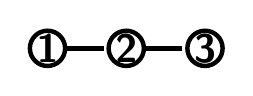
\begin{tikzpicture}[shorten >=1pt, auto, node distance=3cm, ultra thick,main node/.style={circle,draw,minimum size=.4cm,inner sep=0pt]}]%fill=black,
\begin{scope}[every node/.style={font=\sffamily\Large\bfseries}]
\node[main node] (v1) at (0,0) {1};
\node[main node] (v2) at (1,0) {2};
\node[main node] (v3) at (2,0) {3};
%\node[main node] (v) at (,) {};
\end{scope}
\begin{scope}
\draw  (v1) edge node{} (v2);
\draw  (v2) edge node{} (v3);
%\draw  (v) edge node{} (v);
\end{scope}
\end{tikzpicture}
\caption*{Ścieżka $S$.}
%\end{wrapfigure}
\end{figure}

\paragraph{A6} Dla ścieżki o $3$ wierzchołkach
\begin{enumerate}[label=\alph*)]
\item Wyznacz wszystkie wartości własne jej macierzy przyległości, rozwiązując układ równań powstały z warunku: $A\bar{x}=\delta \bar{x}$

\textbf{Odpowiedź: }\begin{align*}
& A=\begin{bmatrix}
0&1&0\\1&0&1\\0&1&0
\end{bmatrix}\rightarrow \begin{bmatrix}
0&1&0\\1&0&1\\0&1&0
\end{bmatrix} \begin{bmatrix}
x\\y\\z
\end{bmatrix} = \begin{bmatrix}
x\lambda \\y\lambda \\z\lambda 
\end{bmatrix}
\end{align*}

\item Dla każdej z trzech wartości własnych wyznacz przykładowy wektor własny jej odpowiadający.
\item Wyznacz powyższe wektory własne tak, aby tworzyły bazę ortogonalna. 
\end{enumerate}

\paragraph{A7} Uzasadnij, że nie istnieją takie grafy na siedmiu wierzchołkach, że spektrum (czyli wszystkie wartości własne wraz z krotnościami) ich macierzy przyległości jest następujące:
\begin{enumerate}[label=\alph*)]
\item $2,\ 2,\ 1,\ 1,\ -3,\ -3,\ -3;$

\textbf{Odpowiedź: }Zgodnie z wzorami podanymi na wykładzie:
\begin{enumerate}[label=\arabic*.]
\item $\mathsf{Tr}[A]=0=\sum_{i=1}^n\lambda _i$ to w tym przypadku: $2+2+1+1-3-3-3 = -3$
\item $\mathsf{Tr}[A^2]=\sum_{i=1}^n\deg (i)=2|E|=\sum_{i=1}^n\lambda ^2_i$ to w tym przypadku: $4+4+1+1+9+9+9=37$ 
\item $\mathsf{Tr}[A^3]=6 \{\underset{Liczba}{\#} K_3 \subseteq G\}=\sum_{i=1}^n\lambda ^3_i$ to w tym wypadku: $8+8+1+1-27-27-27=-63$ ujemne trójkąty?
\end{enumerate}


\item $\sqrt{20},\ 4,\ 2,\ 0,\ -3,\ -3,\ -\sqrt{20};$

\textbf{Odpowiedź: }
\todo[inline,color=red]{ZROBIĆ ZADANIE.}
\item $2,\ 2,\ 0,\ 0,\ -4$.

\textbf{Odpowiedź: }Za mało wartości.
\end{enumerate}


$$\mathsf{Tr}[A]=\sum_{i=1}^n a_{i,i}$$
\begin{fact*}[Słasność śladu]
$$\mathsf{Tr}[ABC]=\mathsf{Tr}[CAB]=\mathsf{Tr}[BAC]$$
\end{fact*}
\begin{align*}
&\mathsf{Tr}[A^k]=\mathsf{Tr}[V \Lambda V^{-1}]=\mathsf{Tr}[\Lambda ^k]=\sum_{i=1}^n\lambda_i^k\\
&A=A(G)\\
&\mathsf{Tr}[A]=0=\sum_{i=1}^n\lambda _i\\
&\mathsf{Tr}[A^2]=\sum_{i=1}^n\deg (i)=2|E|=\sum_{i=1}^n\lambda ^2_i\\
&\mathsf{Tr}[A^3]=6 \{\underset{Liczba}{\#} K_3 \subseteq G\}=\sum_{i=1}^n\lambda ^3_i
\end{align*}

\subsection{Zadania Domowe B}
\paragraph{B1} Rozwiązując równanie $\bar{\bar{A}}\bar{x} = \lambda \bar{x}$, wyznacz spektrum i bazę (nie musi być ortogonalna) wektorów własnych macierzy przyległości grafu $K_{2,3}$.

\paragraph{B2} Znajdź wyrazy macierzy $A^3$ dla grafu $K_n$ metodą kombinatoryczną, tzn. licząc spacery długości 3.

\paragraph{B3} Skorzystaj z faktu, że dla grafu $K_n$ zachodzi $A = J - I$, Znajdź wszystkie wyrazy macierzy $A^4$. Na tej podstawie (i na podstawie wyznaczonego na ćwiczeniach spektrum grafu $K_n$) sprawdź, że rzeczywiście $\mathsf{Tr}(A^4) = \sum ^n _{i=1}\lambda ^4$.

\paragraph{B4} Ślad trzeciej potęgi macierzy przyległości pewnego grafu $G$ wynosi $t$. Ile trójkątów znajduje się w grafie $G$? Dlaczego?

\paragraph{B5} Pewien 3–regularny graf $G$ zawiera dokładnie jeden trójkąt, a $\mathsf{Tr}(A^5) = 90$. Ile cykli o długości $5$ zawiera $G$?

\paragraph{B6} Znajdź $A^{10}$ i $A^{11}$ dla pełnego grafu dwudzielnego $K_{n,m}$.

\paragraph{B7} Załóżmy, że graf $G$ jest niepusty. Czy możliwe jest, żeby
\begin{enumerate}[label=\alph*)]
\item wszystkie wyrazy na przekątnej $A^2$ były równe zero?
\item na przekątnej macierzy $A^3$ pojawiła się jedynka?
\item na przekątnej macierzy $A^3$ pojawiła się dwójka?
\item wszystkie wyrazy na przekątnej $A^3$ były równe zero?
\item dokładnie jeden wyraz na przekątnej $A^3$ był różny od zera?
\end{enumerate}

\paragraph{B8} Znajdź wartości własne i ortonormalny system wektorów własnych dla macierzy przyległości grafu $K_2$. Korzystając z tej bazy, wyznacz $A^k$ dla dowolnego $k \geq 1$.

\paragraph{B9}
\begin{enumerate}[label=\alph*)]
\item Wyznacz bazę ortogonalną macierzy przyległości grafu $K_3$.
\item Wyznacz $A^{123}$ dla grafu $K_3$, Korzystając z poprzedniego podpunktu.
\end{enumerate}

\paragraph{B10} Wyznacz wartości własne i ortonormalny system wektorów własnych dla grafu $G$ na pięciu wierzchołkach, który ma dwie składowe: jedną izomorficzną z $K_3$ i drugą izomorficzną z $K_2$. Korzystając z tej bazy, wyznacz $A^{100}$.

\paragraph{B11} Macierz przyległości $A$ pewnego $10$-regularnego grafu na $20$ wierzchołkach spełnia równanie $$A^2 = 10J - 10A$$ Wyciągnij jak najwięcej wniosków o spektrum macierzy $A$. Przypominamy, że $J$ oznacza macierz, której wszystkie wyrazy są jedynkami.
\todo[inline,color=red]{ZROBIĆ ZADANIE.}

\paragraph{B12} Na podstawie wyglądu macierzy $A^3$ wyznaczonej dla grafu $K_{n,n}$ w zadaniu domowym, napisz równanie macierzowe, w którym $A^3$ jest wyrażona za pomocą $A$. Korzystając z otrzymanego równania macierzowego, wyznacz wszystkie wartości własne $K_{n,n}$ (wraz z krotnościami).

\paragraph{B13} oceń poprawność każdego z poniższych zdań. W każdym przypadku poprzyj odpowiedź, w zależności od potrzeb, uzasadnieniem ogólnym, przykładem lub kontrprzykładem. W wszystkich podpunktach wartości własne dotyczą macierzy przyległości rozważanego grafu,
\begin{enumerate}[label=\alph*)]
\item  Istnieje graf, dla którego wszystkie wartości własne są takie same.
\item  Istnieje graf, którego najmniejszą wartość własna jest dodatnia.
\item  Istnieje graf $3$–regularny, którego spektrum wygląda tak: $2, 2, 2, 0, 0, . . . , 0, 0, -3, -3$.
\item  Jeżeli w spektrum grafu $4$–regularnego wartość własna $4$ ma krotność $3$, to graf ten jest nie Spójny.
\item  Jeżeli graf $4$–regularny ma $3$ składowe, to w jego spektrum wartość własna $4$ ma krotność co najmniej $3$.
\item  Jeżeli w spektrum grafu $G$ największa wartość własna jest większa od wszystkich pozostałych, to graf $G$ jest nie Spójny.
\end{enumerate}

\paragraph{B14} Niech 
$$B=\begin{bmatrix}
-1&-4\\
2&5
\end{bmatrix}$$
Wyznacz $B^{96}$, Korzystając z faktu, że własność $Z^{-1}AZ = \Lambda$ zachodzi dla każdej macierzy, która ma bazę wektorów własnych ($A$ nie musi być macierzą przyległości grafu).

\paragraph{B15} Znajdź liczbę wszystkich spacerów o długości $100$ w ścieżce o trzech wierzchołkach, które zaczynają się w jednym końcu ścieżki i kończą w drugim końcu ścieżki
\begin{enumerate}[label=\alph*)]
\item kombinatorycznie
\item używając ortonormalnej lub ortogonalnej bazy wektorów własnych i własności, że $Z^{-1}AZ = \Lambda $.
\end{enumerate}

\subsection{Zadania}
\paragraph{Zad.1} Dlaczego Jeśli spektrum macierzy przyległości grafu $G$ jest symetryczne, to $G$ jest dwudzielny? Prawdziwa jest również zależność w drugą stronę, ale uzasadnienie tego faktu pozostawiamy zainteresowanym życiem grafów.
\paragraph{Zad.2} Wyznacz spektrum macierzy przyległości cyklu $C_4$, nie Korzystając z (podanego na wykładzie) rozwiązania równania $\bar{\bar{A}}\bar{x} = \lambda \bar{x}$.
\paragraph{Zad.3} Wyznacz spektrum i bazę wektorów własnych dla $K_3$.
\paragraph{Zad.4}
\begin{enumerate}[label=\alph*)]
\item Załóżmy, że znamy spektrum i bazę wektorów własnych dla macierzy przyległości każdej składowej niespójnego grafu $G$. Jak wyznaczyć szybko spektrum i bazę wektorów własnych dla macierzy przyległości grafu $G$?
\item Wyznacz spektrum i bazę wektorów własnych grafu złożonego z wierzchołkowo rozłącznych $K_3$ i $P_3$ oraz z wierzchołka izolowanego. można wykorzystać bazę wektorów własnych dla $P_3$, wyznaczoną w zadaniu domowym.
\end{enumerate}

\paragraph{Zad.5} Macierz przyległości pewnego grafu o $3$ krawędziach spełnia równanie $A^3 = A^2 + 2A$. Wyciągnij jak najwięcej wniosków o spektrum macierzy $A$.
\paragraph{Zad.6} Korzystając z faktu, że $A = J - I$ dla grafu $K_n$,
\begin{enumerate}[label=\alph*)]
\item wyznacz spektrum macierzy $A$.
\item wyznacz $A^3$. Przez $J$ oznaczamy macierz złożoną z samych jedynek, $I$ jest macierzą jednostkową.
\end{enumerate}


%--------------------------------------------------